\chapter{Wstęp}

Rozpowszechnione algorytmy sztucznej inteligencji wspomagające pracę inżynierów dźwięku i kompozytorów
można podzielić na trzy główne kategorie~\cite{analysis_generative}~\label{traditional_algos}:

\begin{enumerate}
    \item algorytmy generujące symboliczny zapis muzyki (nuty lub dane MIDI) (\ref{fig:lamus_notes}),~\cite{zhang2023language},
    \item algorytmy generujące gotowy plik audio na podstawie opisu użytkownika (\ref{fig:riffusion_spectro}).
    \item algorytmy symulujące brzmienie instrumentów muzycznych~\cite{engel2017neural}.
\end{enumerate}

Pierwsza grupa algorytmów znana jest już od lat 80, gdyż zagadnienie generowania zapisu symbolicznego wymaga mniej mocy obliczeniowej niż wytworzenie pełnego pliku audio.
Powszechnie wykorzystywana jest w nich teoria muzyki, pozwalająca określić matematyczne relacje występujące w rytmach, melodiach i progresjach akordów.
Wiedza dotyczącą teorii muzyki pozwala na wyznaczenie możliwej przestrzeni stanów, w której generowana jest kompozycja,
natomiast modele matematyczne takie jak łańcuchy Markowa służą za mechanizmy decyzyjne.

\begin{figure}[H]
    \centering
    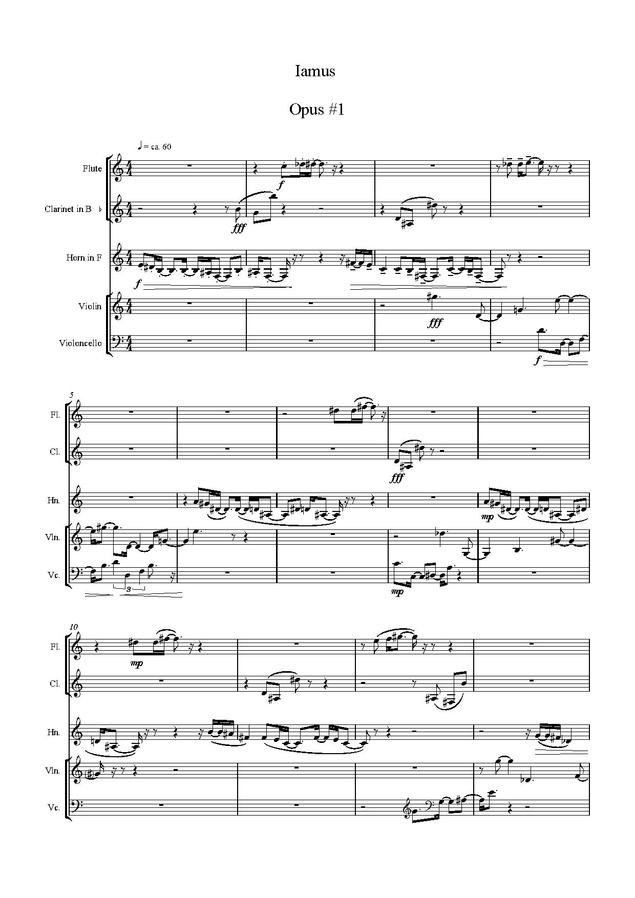
\includegraphics[width=0.4\linewidth]{rys01/lamus_notes.jpg}
    \caption{
      Zapis nutowy utworu \textit{Opus One},
      wygenerowany przez komputer \textit{Lamus}.
    }\label{fig:lamus_notes}
\end{figure}

Druga grupa algorytmów, generująca pliki audio, bazuje na klasie algorytmów
wywodzących się ze \textit{Stable Diffusion}~\cite{stablediffusion}.
Modele generujące pliki audio zgodne z opisem tekstowym 
(przykładowo \texttt{,,smutny jazz''} bądź \texttt{,,muzyka taneczna w stylu Depeche Mode''})
szkolone są w taki sam sposób jak algorytmy \textit{stable diffusion},
dane treningowe składają się z obrazów spektrogramów~\cite{riffusion}. 
Po trenowaniu, model jest wstanie wygenerować spektrogram zawierający
utwór muzyczny zgodny z poleceniem użytkownika (\ref{fig:riffusion_spectro}).
Wygenerowany przez model spektrogram jest konwertowany 
do sygnału dżwiękowego za pomocą odwrotnej transformaty Fouriera.

\begin{figure}[H]
    \centering
    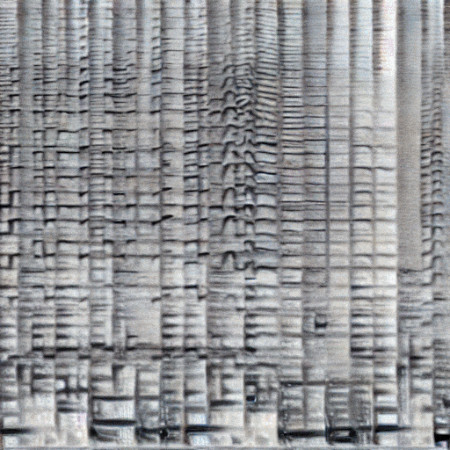
\includegraphics[width=0.4\linewidth]{rys01/riffusion_spectro.jpg}
    \caption{
      Przykładowy spektrogram wygenerowany przez algorytm \textit{Stable Riffusion}
      dla danych wejściowych \texttt{funk bassline with a jazzy saxophone solo}.
    }\label{fig:riffusion_spectro}
\end{figure}

Trzecia grupa algorytmów, symulowanie brzemienia instrumentów muzycznych, najczęściej wykorzystuje sieci
neuronowe trenowane na brzmieniu prawdziwych instrumentów~\cite{engel2017neural}~\cite{engel2020ddsp}. 
Tego typu algorytmy pozwalają symulowanie instrumentów o złożonych barwach, takich jak instrumenty
smyczkowe lub dęte oraz na płynne przechodzenie między brzmieniami różnych instrumentów muzycznych.

% TODO: check later
% https://github.com/Kinyugo/msanii

Metody opisane w rozdziale~\ref{traditional_algos} można porównać pod względem ich przydatności
dla użytkownika końcowego, czyli osoby zajmującej się produkcją nagrań muzycznych. Metoda pierwsza, 
generowanie zapisu symbolicznego, może wydawać się mniej zaawansowana niż generowanie całych plików dźwiękowych.
Jednakże, z perspektywy użytkownika, zapis symboliczny jest bardziej praktyczny,
ponieważ możliwe jest zaimportowanie go do programu DAW i późniejsza modyfikacja zapisu nutowego.
Obecnie dostępne modele generujące pełne nagrania z muzyką nie umożliwiają
szczegółowego edytowania parametrów wygenerowanego dźwięku, ponieważ operują bardzo wysokopoziomowo 
-- syntezują muzykę na podstawie opisu słownego. Podobne problemy występują również podczas wykorzystywania
algorytmów z grupy trzeciej, głębokie sieci neuronowe nie są przystosowane do ręcznej modyfikacji przez użytkownika.

Podsumowując, wykorzystanie wygenerowanego przez komputer zapisu nutowego jest proste, ze względu na symboliczną naturę zapisu.
Wykorzystanie wygenerowanego przez komputer dźwięku jest ograniczone ze względu na fakt, że do generowania złożonych sygnałów dźwiękowych wykorzystywane są techniki takie jak głębokie sieci neuronowe, w których utrudniona jest dokładna kontrola nad konkretnymi parametrami funkcjonowania sieci.

Niniejsza praca sugeruje nową metodę podejścia do problemu generowania sygnałów dźwiękowych,
którego nie da się zaklasyfikować do żadnej z wyżej wymienionych~(\ref{traditional_algos}) dziedzin komputerowej kompozycji muzycznej.
Graf przetwarzania sygnałów wytworzony przez algorytm implementowany w ramach pracy magisterskiej jest przepisem na gotowy elektroniczny instrument muzyczny,
który może być wykorzystany w programie do komponowania muzyki. Algorytm nie generuje bezpośrednio sygnału dźwiękowego, lecz tworzy
graf przetwarzania sygnałów, który jest zrozumiały dla użytkownika i pozwala na precyzyjne dostosowanie parametrów syntezy.
Tego typu proces generowania grafów przetwarzania sygnałów dźwiękowych może być porównany z procesem projektowania instrumentu muzycznego.

Modyfikowanie ścieżki przetwarzania sygnału jest techniką często wykorzystywaną w muzyce
elektronicznej, do tworzenia dźwięków o interesującej barwie bądź dynamice. Syntezatory dźwięku
dostępne na rynku często wyposażone są w tzw. \textit{patch bay}~(\ref{fig:mother32}), pozwalający na modyfikowanie
grafu przepływu sygnałów wewnątrz syntezatora, bądź połączenie go z zewnętrznym sprzętem muzycznym
bądź elektronicznym.

\begin{figure}[H]
    \centering
    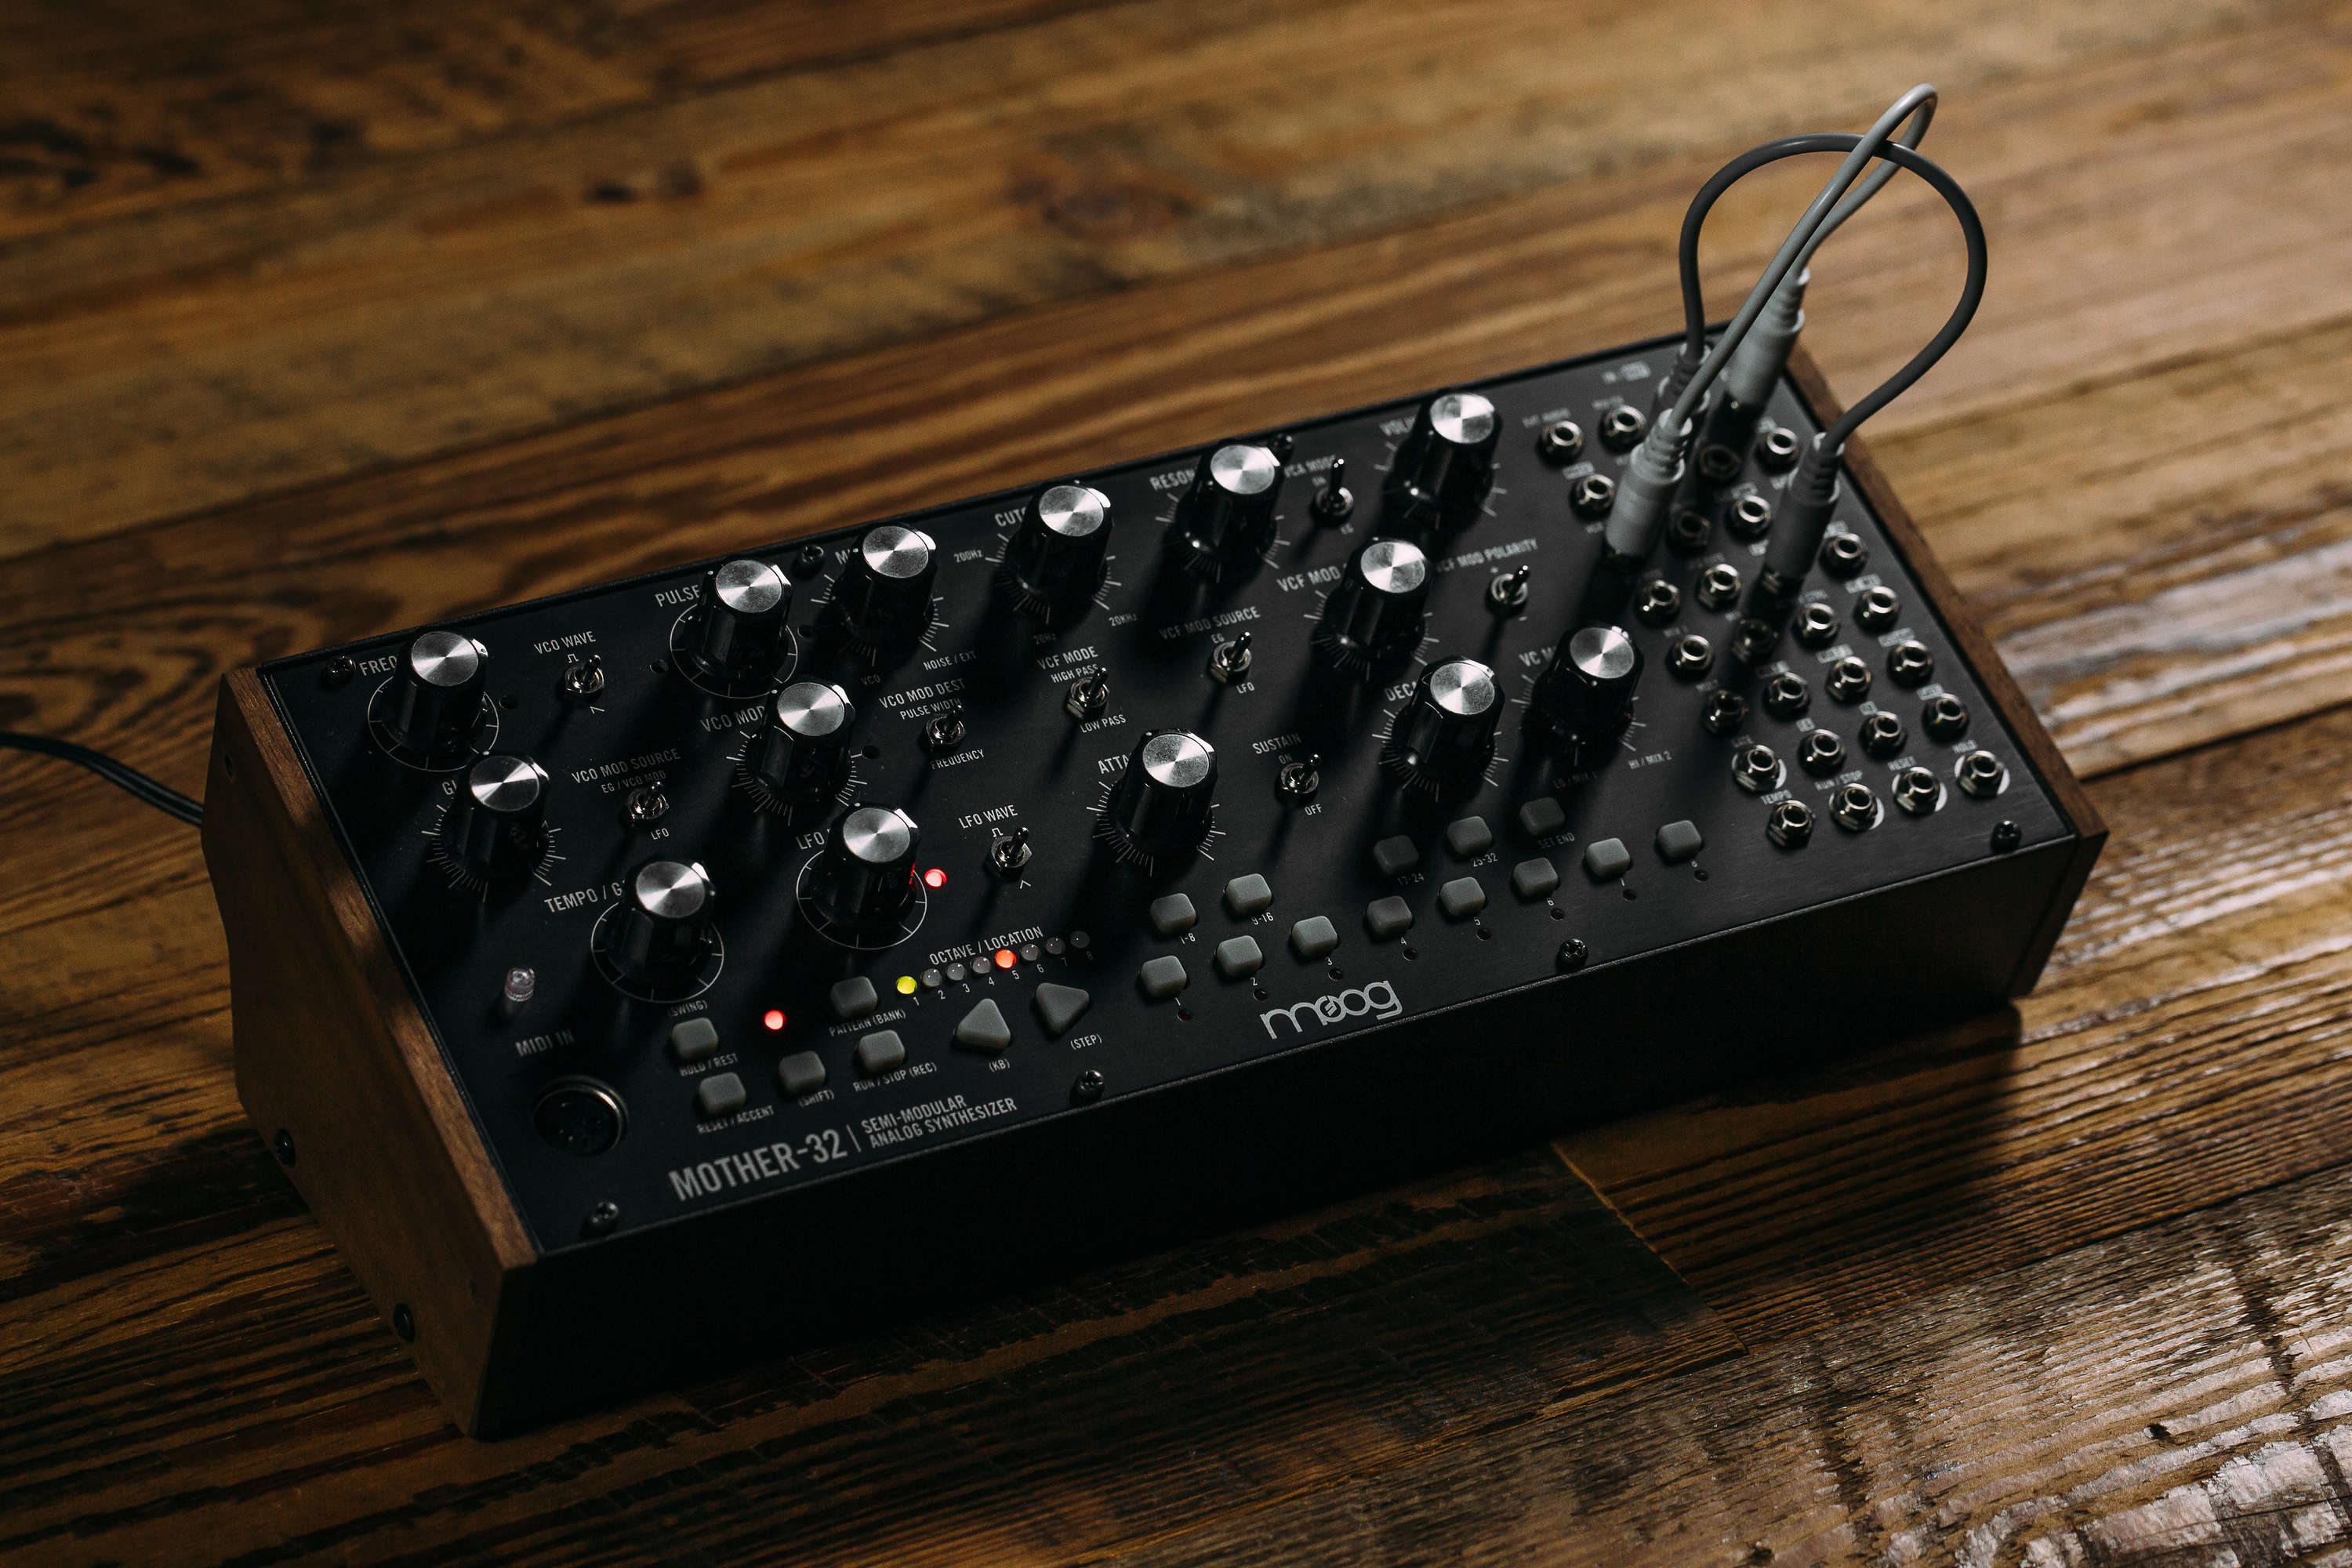
\includegraphics[width=0.7\linewidth]{rys01/mother32.jpg}
    \caption{
      Syntezator \textit{Mother 32} firmy \textit{Moog}, po prawej stronie widoczny
      jest \textit{patch bay} z podłączonymi przewodami, które nadpisują konfigurację
      połączeń między układami generującymi i przetwarzającymi sygnał dźwiękowy.
    }\label{fig:mother32}
\end{figure}


\section{Cel pracy}

Celem pracy jest \textbf{opracowanie algorytmu generacji grafów przetwarzania sygnałów, który
który wykona syntezę próbki dźwięku zadanej przez użytkownika}.
Problem poruszany w pracy można zakwalifikować do grupy zagadnień związanych
z pojęciami \textit{computer-aided design} oraz \textit{generative artificial intelligence}, zastosowanymi w dziedzienie inżynierii dźwięku. Docelowo
zaimplementowany algorytm będzie automatyzował pracę inżyniera dźwięku,
tworząc i konfigurując grafy przetwarzania sygnałów dźwiękowych, dostępne w
programach typu \textit{digital audio workstation}~(\ref{fig:ableton_patch}). Badania obejmują dwa zagadnienia:
\textbf{
\begin{enumerate}\label{research_types}
    \item opracowanie metody generowania grafu przetwarzania sygnałów oraz późniejszej modyfikacji grafu -- jego struktury i parametrów,
    \item dobór funkcji celu, na podstawie której algorytm optymalizujący będzie modyfikował graf przetwarzania sygnałów.
    \item przeprowadzenie badań symulacyjnych, które zweryfikują skuteczność opracowanego algorytmu.
    \item porównanie wyników badań symulacyjnych z pracami naukowymi o podobnej tematyce.
\end{enumerate}
}

\begin{figure}[H]
    \centering
    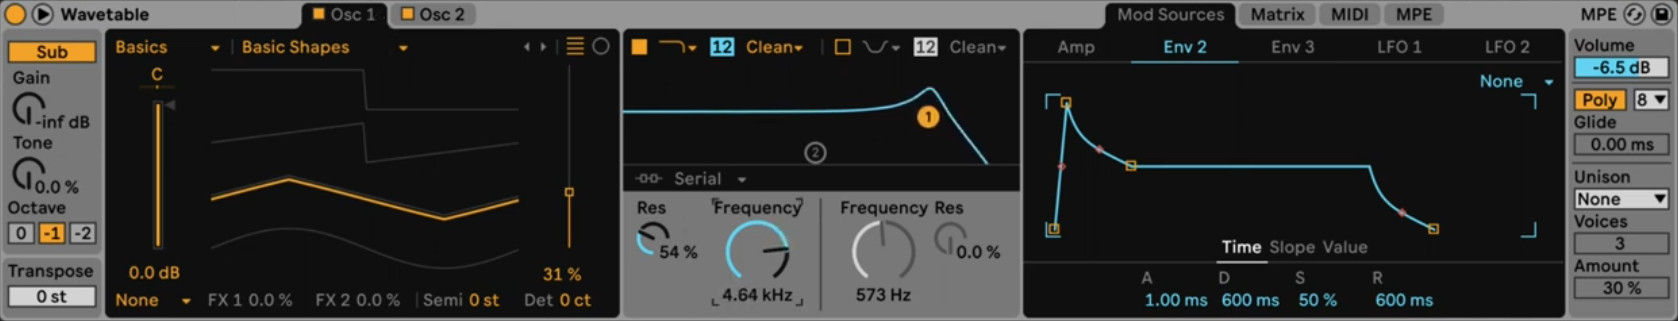
\includegraphics[width=0.8\linewidth]{rys01/ableton_patch.jpg}
    \caption{
      Zbiór parametrów konfigurujących syntezator dźwięku \textit{Wavetable} w programie \textit{Ableton}
    }\label{fig:ableton_patch}
\end{figure}

\subsection{Generowanie grafu przetwarzania sygnałów}

Proces syntezy dźwięku może być przedstawiony jako graf przetwarzania sygnałów, w którym
każdy węzeł wykonuje na sygnale określoną operację.
Przykładowy graf przetwarzania sygnału dla syntezatora analogowego subtraktywnego
przedstawiony jest na schemacie~\ref{fig:minilogue_diagram}.
Pierwsze zagadnienie sprowadza się do opracowania algorytmu pozwalającego na wygenerowanie
grafu przetwarzania sygnałów DSP oraz jego późniejszą modyfikację. Przykładem modyfikacji grafu
może być wprowadzanie do niego nowych źródeł modulacji bądź zmiana algorytmu generującego sygnał.

\begin{figure}[H]
    \centering
    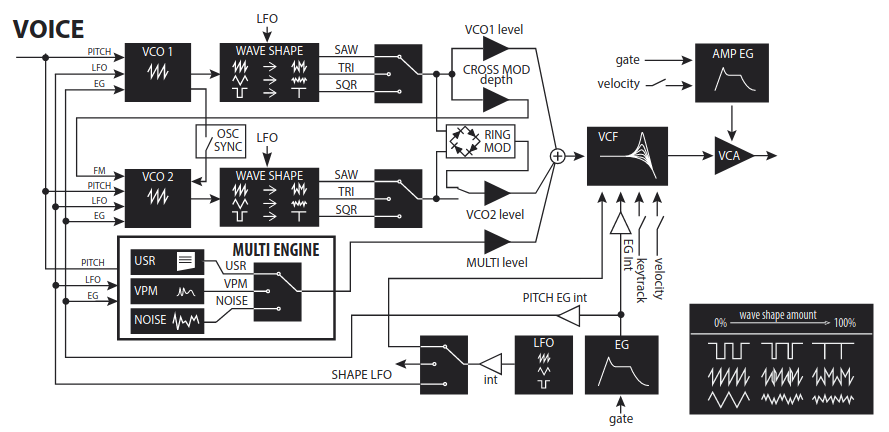
\includegraphics[width=0.8\linewidth]{rys01/minilogue_voice_block_diagram.png}
    \caption{
      Diagram blokowy pojedynczego głosu w syntezatorze 
      \textit{Minilogue xd} firmy \textit{Korg}~\cite{minilogue_diagram}.
    }\label{fig:minilogue_diagram}
\end{figure}

\subsection{Funkcja celu oceniająca podobieństwo barwy dźwieku}

Drugie zagadnienie obejmuje przetestowanie szeregu algorytmów, które można
wykorzystać do zbudowania funkcji celu, która będzie optymalizowana
poprzez~,,dostrajanie'' parametrów i struktury grafu przetwarzania sygnałów dźwiękowych.
% todo: więcej o funkcji celu
Praca proponuje wykorzystanie współczynników cepstralnych sygnału (MFCC) w połączeniu
z dynamicznym skalowaniem czasu (\textit{dynamic time wrapping}, DTW) jako funkcji celu.
Proces wyboru funkcji celu został
opisany w rozdziale~\ref{target_function_chapter}.

\subsection{Problem optymalizacyjny}

W pracy rozwiązywany jest problem optymalizacyjny, w którym
struktura oraz parametry grafu przetwarzania sygnałów dostosowywane
są tak, aby wygenerować zadaną próbkę dźwięku. Tak wytworzony
graf może być wykorzystany jako elektroniczny instrument muzyczny. 

% Następnie, dla danego układu $N$ węzłów przetwarzania oraz dla macierzy połączeń $C$, 
% należy rozwiązać następujący problem optymalizacji, należy rozwiązać problem
% maksymalizacji funkcji opisanej równaniem~\ref{eq:target_function} dla
% parametrów wszystkich wejść $i_j$ oraz $o_j$, które nie są połączone bezpośrednio
% pomiędzy węzłami.




\section{Zakres pracy, plan badań}\label{chap:thesis_scope}

\subsection{Metody generowania grafu przetwarzania sygnałów oraz późniejsza modyfikacja grafu}

Głównym problemem przy generowaniu grafu przetwarzania sygnałów są ograniczenia nałożone na strukturę grafu,
które należy spełnić, by graf był logicznie interpretowalny jako łańcuch przetwarzania sygnałów.
Graf musi być grafem skierowanym, który nie zawiera pętli o dodatnim sprzężeniu zwrotnym.
% Struktura grafu powinna być możliwie jak najbardziej przejrzysta dla użytkownika. 
Automatyczna ewolucja może dążyć w kierunku wykorzystania nadmiarowej liczby
bloków przetwarzania sygnału, jeśli funkcja celu nie będzie zawierała kary za zbyt złożone grafy.
Podobne prace~\cite{evolutionary_puredata} wykorzystują podejście oparte o 
\textit{mixed-typed carthesian genetic programming}, które będzie punktem startowym dla pracy.
Finalnie, badania dążą do wyznaczenia algorytmu o następujący właściwościach:

\begin{enumerate}
    \item algorytm generuje grafy będące logicznie spójnymi łańcuchami przetwarzania dźwięku (skierowany, bez pętli o dodatnim sprzężeniu zwrotnym w natężeniu sygnału),
    \item algorytm maksymalizuje wykorzystanie poszczególnych bloków przetwarzania w grafie, co minimalizuje finalny rozmiar grafu, czyniąc go bardziej czytelnym,
    \item generowany graf posiada reprezentację umożliwiającą wykonanie krzyżowania dwóch grafów przetwarzania sygnału. Graf będący wynikiem krzyżowania nadal musi być poprawnym grafem przetwarzania sygnału.
\end{enumerate}

\noindent
Elementami grafu przetwarzania sygnałów są używane powszechnie w syntezie dźwięku algorytmy:

\begin{enumerate}
  \item modulacja FM~\cite{spectral_audio_processing}~\cite{computational_music_synthesis},
  \item synteza subtraktywna~\cite{computational_music_synthesis}~\cite{digital_filters},
  \item algorytmy \textit{physical modeling}~\cite{lisp_synthesis}~\cite{computational_music_synthesis},
  \item symulacja efektu pogłosu/echa~\cite{reverb}~\cite{freeverb}.
\end{enumerate}

\subsection{Dobór funkcji błędu: różnica między wygenerowanym a docelowym sygnałem dźwiękowym}

Funkcja celu poszukiwana w ramach projektu musi określać, jak dobrze sygnał wygenerowany przez
graf przetwarzania sygnałów pokrywa się z sygnałem docelowym. Porówanie sygnałów musi skupiać się
na cechach sygnału, które są najbardziej słyszalne dla ludzkiego ucha. Jednocześnie funkcja nie powinna
,,karać'' sygnałów, które są względem siebie przesunięte w fazie. Wśród algorytmów, które zostały wybrane
do przetestowania w ramach projektów zawarte są:

\begin{enumerate}
  \item algorytmy porównywania sygnałów oparte o transformatę Fouriera~\cite{sliding_fourier}~\cite{mfcc},
  \item techniki wykorzystywane do generowania~,,cyfrowych podpisów'' sygnałów dźwiękowych (\textit{sound fingerprinting})~\cite{computer_vision_music_identification},
  \item algorytmy wykrywające spadek jakości dźwięku z perspektywy psychoakustycznej~\cite{peaq}~\cite{frechet_audio_distance}.
\end{enumerate}

\section{Struktura i zawartość pracy}

% Praca podzielona jest na następujące części:

Rozdział \textbf{Definicja problemu} formalizuje i opisuje problem optymalizacyjny rozwiązywany w pracy.
W rozdziale \textbf{Analiza i wybór funkcji celu} opisano proces porównywania funkcji z dziedziny przetwarzania sygnałów,
które pozwalają określić jak podobna jest barwa dźwięku dwóch sygnałów dźwiękowych i
uzasadniono wybór funkcji celu, która została zastosowana w pracy.
Rozdział \textbf{Algorytm rozwiązania} opisuje algorytm wykorzystany do rozwiązania problemu
zdefiniowanego w rozdziale~\ref{chap:problem_definition}.
W rozdziale \textbf{Implementacja grafu przetwarzania sygnałów} opisane zostało zaimplementowane w ramach pracy środowisko eksperymentalne,
pozwalające na wytwarzanie grafów przetwarzania sygnałów o dowolnej strukturze.
Przedstawione są w nim również zaimplementowane algorytmy syntezy i przetwarzania sygnałów dźwiękowych.
Rozdział \textbf{Wyniki badań} opisuje proces badawczy, w którym narzędzia wytworzone w
rozdziałach~\ref{dsp_graph_chapter} oraz~\ref{target_function_chapter}
zostały wykorzystane do automatycznego wytworzenia grafu DSP, który naśladuje barwę zadanej próbki dźwięku.
Porównuje uzyskane wyniki z podobną pracą badawczą~\cite{evolutionary_puredata}.
Rozdział \textbf{Analiza wyników, możliwe drogi dalszego rozwoju} podsumowuje uzyskane wyniki badań, podejmuje dyskusję nad ogólną skutecznością i przydatnością zaimplementowanego rozwiązania oraz
kreśli potencjalne drogi dalszego rozwoju prac badawczych w podobnej tematyce. W czasie, gdy niniejsza praca była tworzona, zostały opublikowane badania
dotyczące podobnego problemu~\cite{ieee_synth_programming}, rozdział podejmuje dyskusję o różnicach w podejściu do problemu oraz potencjalnych
zalet i wad każdego z podejść.

